\documentclass[revtex4-2]{mpltx}
\usepackage{physics}
\newcommand*\cs[1]{\texttt{\textbackslash #1}}
\newcommand*\env[1]{\textit{\texttt{#1}}}
\newcommand*\code[1]{\texttt{#1}}
\newcommand*\file[1]{\textbf{\texttt{#1}}}


\begin{document}
\title{康普顿散射}
\author{方尤乐}

\emailphone{eden@stu.pku.edu.cn}{(86)15313960363}
\affiliation{北京大学物理学院\quad 学号: 2000012416}
\begin{abstract}
    康普顿效应源于电子对高能光子的非弹性散射,反映了光具有波粒二象性。
    本实验以 ${}^{137}$Cs 为放射源,测定了 0.662 MeV $\gamma$ 射线被铝棒散射后的能量及相对微
    分散射截面,测量了它们在不同散射角下的大小。实验结果表明,
    散射光子能量及相对微分散射截面与理论计算的结果基本一致,从而验证了康普顿效应的理论公式,证实了光的波粒二象性。
\end{abstract}
\keywords{康普顿散射,散射截面,闪烁体探测器}
\maketitle
\section{引言}
20 世纪初,人们通过众多实验发现,被物质散射后的 X 射线能量减小;
这违背了光的经典波动学说的预言——散射波的能量应当与入射波一致。
1923 年,康普顿采用光量子假定,结合狭义相对论的动力学,成功解释了散射能量的变化。
康普顿提出了 X 射线被散射后能量减小是源于电子对高能光子的非弹性散射,
它反映了光具有波粒二象性。1928 年,Oskar Klein 和 Yoshita Nishina 根据量子电动力学(QED)推导出了康普顿散射的微分截面。
Klein–Nishina 公式是 QED 的最早成果之一,它在低能极限下等同于经典的弹性散射(汤姆逊散射),
而在高能情形下给出康普顿散射的结果。

康普顿散射已成为研究基本粒子结构的一个重要方法。本实验以 ${}^{137}$Cs 为放射源,
利用闪烁体探测器测定散射光子的能谱,来分析散射光子的能量及相对微分散射截面随
散射角 $\theta$ 的变化,以验证康普顿散射理论计算结果。
\section{理论}\label{sec:theory}
参见 [3], 考虑高能极限,即光子能量远大于电子束缚能,此时电子近似是自由的;
由相对论性能动量守恒,光子能量 $\epsilon = h\nu$,可得
\begin{align}
    \label{eq:3}h\nu'=\frac{h\nu}{1+\frac{h\nu}{mc^2}(1-\cos\theta)}
    \quad \Rightarrow \quad \frac{\nu}{\nu'}=1+\alpha(1-\cos\theta),\alpha=\frac{h\nu}{mc^2}
\end{align}
其中 $\nu'$ 为散射光子频率,$\theta$ 为散射角,$m\sim 0.511\ \mathrm{MeV/c^2}$ 为电子质量,$c$ 为光速。

Klein–Nishina 公式给出了散射的微分截面
\begin{align*}
    &\frac{\mathrm{d}\sigma}{\mathrm{d}\Omega}=\frac{r_0^2}{2}\left(\frac{\nu'}{\nu}\right)^2\left(\frac{\nu'}{\nu}+\frac{\nu}{\nu'}-\sin^2\theta\right)\\
    &   =\frac{r_0^2}{2}\left(\frac{1}{1+\alpha(1-\cos\theta)}\right)^2
    \left(\frac{1}{1+\alpha(1-\cos\theta)}+(1+\alpha(1-\cos\theta))-\sin^2\theta\right)\\
    &   =\frac{r_0^2}{2}\left(\frac{1}{1+\alpha(1-\cos\theta)}\right)^2\left(\frac{1+\cos^2\theta}{2}\right)
    \left(1+\frac{\alpha^2(1-\cos\theta)^2}{(1+\cos^2\theta)(1+\alpha(1-\cos\theta))}\right)
\end{align*}
在真实测量的结果中,微分散射截面可以被表示为
\begin{align}
    \label{eq:1}\frac{\mathrm{d}\sigma}{\mathrm{d}\Omega}
    \propto\frac{N(\theta)}{R(e)\eta(e)},\quad e=e(\theta)
\end{align}
其中 $N(\theta)$ 为散射光子数计数,峰总比 $R(e)$ 和探测效率 $\eta(e)$ 为探测器的属性。
本实验中,对 $20^\circ,40^\circ,60^\circ,80^\circ,100^\circ,120^\circ$ 六个散射角,
测量了散射谱和本底谱,计算峰值所对应的道数,来得到散射光子的能量 $e$。
为了计算微分散射截面,约定计算散射谱中 $>1/3$ 峰值的道数区间的总面积减去本底谱相同道数区间总面积,以减小本底光子对测量结果的影响。
由于它正比于 $N(\theta)$,所以可以利用 \eqref{eq:1} 计算相对微分散射截面:
\begin{align}
    \label{eq:4}\frac{(\dd\sigma/\dd\Omega)_\theta}{(\dd\sigma/\dd\Omega_0)_{\theta_0}}=\frac{N(\theta)/R(e)/\eta(e)}{N(\theta_0)/R(e_0)/\eta(e_0)}
\end{align}
\section{实验装置}
本实验使用 ${}^{137}$Cs 放射源出射 $0.662\ \mathrm{MeV}$ 能量的光子,经过铝棒散射后,被 NaI(Tl) 闪烁体探测器探测,闪烁体探测器可以以散射棒为中心旋转,来改变散射角 $\theta$。
实验装置如图 \ref{fig:1} 所示。
\begin{figure}[htbp]
    \centering
    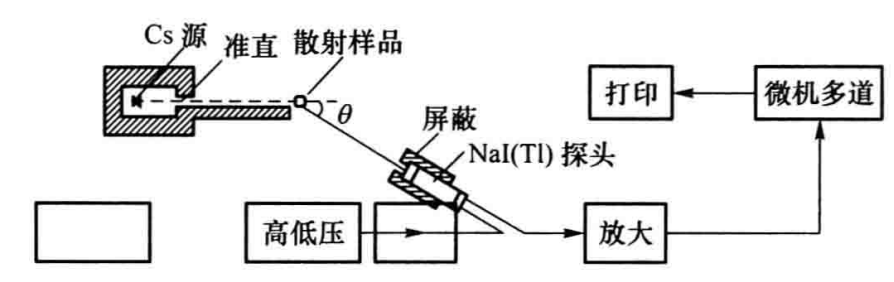
\includegraphics[width=0.6\textwidth]{1.png}
    \caption{实验装置示意图}
    \label{fig:1}
\end{figure}

实验过程中,利用 ${}^{137}$Cs 的 0.662 MeV、 ${}^{60}$Co 源的 1.17 MeV 和 1.33 MeV 的 $\gamma$ 射线,来标定能量刻度。
测量散射谱和本底谱的时候,约定设置测量统计光子数量的时间都为十分钟,
测量本底谱的时候,撤去铝棒,再在各个角度进行测量。

\section{结果及讨论}
\subsection{能量标定}
利用 ${}^{137}$Cs 的 0.662 MeV、 ${}^{60}$Co 源的 1.17 MeV 和 1.33 MeV 的 $\gamma$ 射线,来标定能量刻度。 $\gamma$ 射线的能量与峰值道数数据如表 \ref{tab:1} 所示。
\begin{table}[htbp]
    \centering
    \caption{射线的能量与峰值道数数据}
    \label{tab:1}
    \begin{tabular}{cccc}
        \hline
        能量 $E$/MeV & 0.662 & 1.17 & 1.33 \\
        \hline
        峰值道数 $x$ & 477 & 844 & 964 \\
        \hline
    \end{tabular}
\end{table}

这三个数据的 Pearson 相关系数为 0.99997,说明它们之间的线性关系非常好,可以用线性拟合来标定能量刻度:
\begin{align}
    \label{eq:2}E\mathrm{/MeV}=0.001375 x +  0.007010
\end{align}
\subsection{峰值测量,确定散射光子能量}
测量 $20^\circ,40^\circ,60^\circ,80^\circ,100^\circ,120^\circ$ 六个散射角的散射谱和本底谱。
六个散射角对应的峰值道数和能量如表 \ref{tab:2},峰值能量与散射角的关系如图 \ref{fig:4} 所示。
\begin{table}[htbp]
    \centering
    \caption{六个散射角对应的峰值道数和能量}
    \label{tab:2}
    \begin{tabular}{ccccccc}
        \hline
        散射角 $\theta$/度 & 20 & 40 & 60 & 80 & 100 & 120 \\
        \hline
        峰值道数 $x$ &  440 &368 &286 &227 &189 &157\\
        能量 $E$/MeV & 0.612 & 0.513 & 0.400 & 0.319 & 0.267 & 0.223 \\
        \hline
    \end{tabular}
\end{table}
\begin{figure}[htbp]
    \centering
    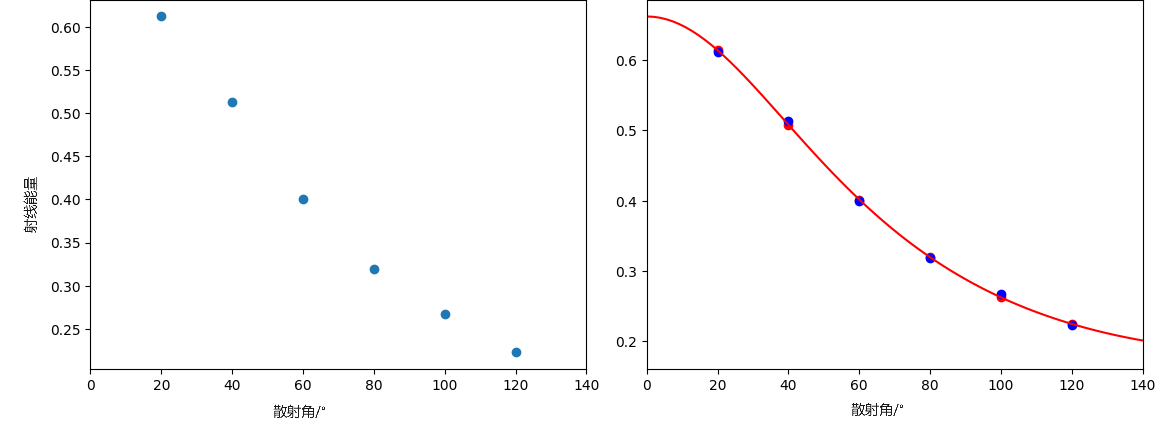
\includegraphics[width=0.9\textwidth]{4.png}
    \caption{六个散射角对应峰值能量,右图中红线是理论预言曲线,蓝点是测量结果}
    \label{fig:4}
\end{figure}

图 \ref{fig:4} 中,蓝点表示六个散射角测得的峰值能量,右图中红线是理论预言曲线,由康普顿散射光子能量公式 \eqref{eq:3} 得到。
可以看到,测量结果与理论预言曲线符合得非常好,说明康普顿散射理论是正确的。散射光子能量与理论值之间的误差约为
$2\%$。误差主要是由于十分钟内闪烁体探测器收集的光子数量有限,峰值位置的测量不够精确。

\subsection{测量计算微分散射截面}
图 \ref{fig:3} 为两个谱相减得到的结果。
\begin{figure}[htbp]
    \centering
    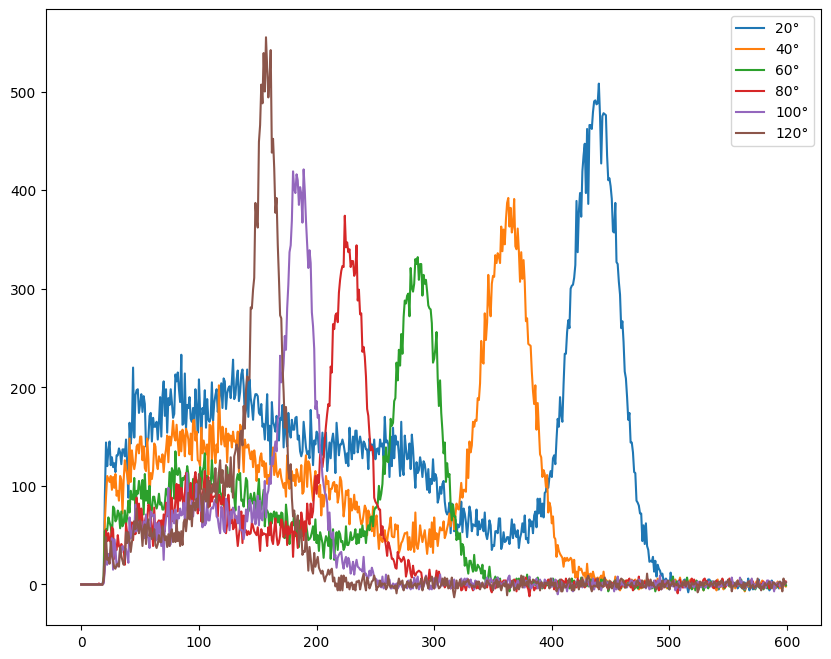
\includegraphics[width=0.8\textwidth]{3.png}
    \caption{散射谱和本底谱相减得到的结果}
    \label{fig:3}
\end{figure}
利用 \eqref{eq:1} 和 \eqref{eq:4} 计算相对散射截面,先利用散射谱中峰值的 $1/3$ 高度来确定要统计的道数区间,
然后计算道数区间内的总面积,
与本底谱对应区间的面积作差,得到的结果如表 \ref{tab:3} 所示。

\begin{table}[htbp]
    \centering
    \caption{峰值 $1/3$ 区间对应的散射谱、本底谱总面积}
    \label{tab:3}
    \begin{tabular}{ccccccc}
        \hline
        散射角 $\theta$/${}^\circ$ & 20 & 40 & 60 & 80 & 100 & 120 \\
        \hline
        散射谱总面积 & 23034 & 17613 & 13411 & 12142 & 12173 & 13811 \\
        本底谱总面积 & 1190 & 583 & 537 & 597 & 694 & 928 \\
        散射谱减去本底谱总面积 $N(\theta)$ & 21844 & 17030 & 12874 & 11445 & 11479 & 12883 \\
        \hline
    \end{tabular}
\end{table}

在计算过程中,引用了近代物理实验课本中给出的 $R(e),\eta(e)$ 数据表;用三次样条插值
来估计六个散射角所对应的 $R,\eta$,并计算相对微分散射截面
\begin{align*}
    &y_\theta \equiv \frac{N(\theta)}{R(e)\cdot\eta(e)} / 10^7 \propto \left.\frac{\dd \sigma}{\dd \Omega}\right|_{\theta}\\
    &\frac{(\dd\sigma/\dd\Omega)_\theta}{(\dd\sigma/\dd\Omega_0)_{\theta_0}}=\frac{N(\theta)/R(e)/\eta(e)}{N(\theta_0)/R(e_0)/\eta(e_0)}=\frac{y_\theta}{y_{\theta_0}}
\end{align*}
\begin{table}[htbp]
    \centering
    \caption{相对微分散射截面}
    \label{tab:4}
    \begin{tabular}{ccccccc}
        \hline
        散射角 $\theta$/${}^\circ$ & 20 & 40 & 60 & 80 & 100 & 120 \\
        \hline
        $y_\theta \equiv   N(\theta)/(R(e)\cdot\eta(e))/ 10^7\propto\dd\sigma/\dd\Omega $ &7.63 & 4.85 & 2.70 & 
        1.86 & 1.54 & 1.50\\
        相对微分散射截面 $y_\theta / y_{\theta_0}$ & 1 &  0.635 & 0.354 & 0.244 & 0.202 &
        0.196\\
        \hline
    \end{tabular}
\end{table}
结果为 \ref{tab:4},与理论计算曲线对比如图 \ref{fig:6} 所示。
\begin{figure}[htbp]
    \centering
    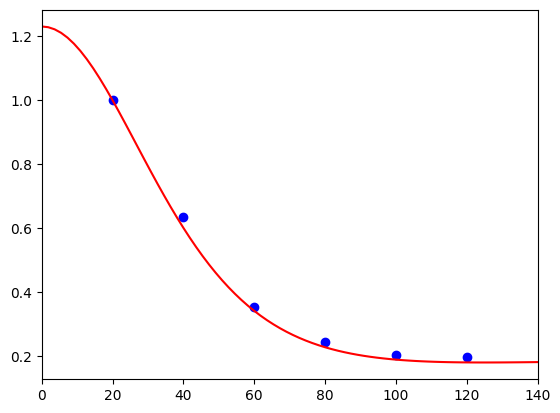
\includegraphics[width=0.8\textwidth]{6.png}
    \caption{相对微分散射截面,右图中红线是理论预言曲线(Klein-Nishina 公式),蓝点是测量计算结果}
    \label{fig:6}
\end{figure}

可以看到,相对微分散射截面的结果与理论预言曲线(Klein-Nishina 公式)大致符合。但是测得的相对微分散射截面略比理论计算结果偏高。
这是因为在测量散射谱的时候,有一部分由于光子射到实验室墙壁再反射回铝棒而发生的散射,也被计入了散射谱中,
而这一部分散射光子没有被计入本底谱中,这导致了散射谱减本底谱的峰值区域总面积偏大,从而测得的相对微分散射截面偏大。

\section{结论}
本实验通过测量 ${}^{137}$Cs 放射源的 $0.662$ MeV $\gamma$ 射线的散射能谱和本底能谱,经过数据处理和计算
,得到了六个散射角下散射光子的能量和相对散射截面,所得结果与康普顿散射的理论预言大致符合。
其中散射光子的能量的误差在 $2\%$ 左右。
这证实了康普顿散射公式 \eqref{eq:3} 的正确性,从而证实了光具有波粒二象性。

相对散射截面的测量结果比理论计算结果偏高,这是因为在测量散射谱的时候,有一部分由于光子射到实验室墙壁再反射回铝棒而发生的散射,也被计入了散射谱中,
而这一部分散射光子没有被计入本底谱中,这导致了散射谱减本底谱的峰值区域总面积偏大,从而测得的相对微分散射截面偏大。


\begin{acknowledgments}
    感谢安刘攀老师对实验注意事项和实验现象的耐心细致的讲解。
\end{acknowledgments}
\bibliography{mybibfile}

\clearpage % 附录前另起一页
\appendix % 附录开始
\section{思考题}\label{app:exercise}
\subsection{分析本实验的主要误差来源,试述有限立体角的影响和减少实验误差的方法}
本实验主要误差来自于误差来自于测量散射谱峰值时的不确定性,在有限的时间(10 分钟)内测得的能谱不构成严格的平滑的曲线,
此外读取道数时存在测量误差,这些都会导致测量的峰值能量有一定的误差。
探测器的峰总比 $R(e)$ 和探测效率 $\eta(e)$ 的不确定性也对实验值误差有贡献。
实验环境中墙壁、其他物体与铝棒的反射也会导致散射谱中一部分背景光子没有被统计到本底谱中,
这也导致了实验值的误差。

此外,探测器测得的是有限立体角范围内的光子,因此实验值不是严格意义上的微分散射截面。
减少实验误差的方法有:减小探测器窗口大小、增加探测器与铝棒的距离、增加测量时间;保证实验环境周围空旷,且实验室封闭不受外界射线干扰。

\section{讨论实验值与理论值不完全符合的原因}
相对散射截面的测量结果比理论计算结果偏高,这是因为在测量散射谱的时候,
有一部分由于光子射到实验室墙壁再反射回铝棒而发生的散射,也被计入了散射谱中,
而这一部分散射光子没有被计入本底谱中,这导致了散射谱减本底谱的峰值区域总面积偏大,
从而测得的相对微分散射截面偏大。


\end{document}